%%%%%%%%%%%%%%%%%%%%%%%%%%%%%%%%%%%%%%%%%%%%%%%%%%
% File stack.tex
% Copyright (c) 2024 Jeffrey K. Bienstadt
%%%%%%%%%%%%%%%%%%%%%%%%%%%%%%%%%%%%%%%%%%%%%%%%%%
\documentclass{article}
\usepackage[T1]{fontenc}
%\usepackage[top=1in,left=.75in, right=.75in, bottom=1in]{geometry}
\usepackage{cprotect}
\usepackage{float}
\usepackage[bottom]{footmisc}
\usepackage{inconsolata}
\usepackage{listings}
\usepackage{microtype}
\usepackage{relsize}
\usepackage{tikz}
\usepackage{xcolor}
\usepackage{hyperref} % use hyperref package last

\usetikzlibrary{calc,shapes.multipart,chains,arrows,quotes}
\tikzset{
  list/.style={ % image of a singly-linked list node
    very thick, rectangle split,
    rectangle split parts=2, draw,
    rectangle split horizontal, minimum size=18pt,
    inner sep=4pt, text=black,
    rectangle split part fill={red!20, blue!20}
  },
  dlist/.style={  % image of a doubly-linked list node
    very thick, rectangle split,
    rectangle split parts=3, draw,
    rectangle split horizontal, minimum size=18pt,
    inner sep=5pt, text=black,
    rectangle split part fill={blue!20, red!20, blue!20}
  },
  dummy/.style={  % Image of a dummy node
    draw,rectangle,minimum size=18pt, fill=orange!80,
    inner sep=0pt, text=black,
    path picture = {
      \draw[black]
      (path picture bounding box.north west) --
      (path picture bounding box.south east)
      (path picture bounding box.south west) --
      (path picture bounding box.north east);
    }
  },
  endlist/.style={
    draw, rectangle, minimum height=18pt, minimum width=30pt, gray, thick, dashed
  }
}

\hypersetup{
  colorlinks=true,
  linkcolor=blue,
  urlcolor=blue,
  pdftitle={An Introduction to the Stack Data Structure},
  pdfauthor={Jeff Bienstadt},
  pdfsubject={Stack},
  pdfkeywords={stack, computing, data structures, C, C++}
}

\lstset{
  basicstyle        = \small\ttfamily,
  keywordstyle      = \color{blue}\textbf,
  commentstyle      = \color{gray}\rmfamily\itshape,
  columns           = fullflexible,
  numbers           = left,
  numberstyle       = \scriptsize\sffamily\color{gray},
  showstringspaces  = false,
  keepspaces        = true
}

\lstnewenvironment{algorithm}[1][] %defines the algorithm listing environment
{
    \lstset{
        mathescape=true,
        frame=tB,
        numbers=left,
        numberstyle=\tiny,
        basicstyle=\small\em,
        keywordstyle=\color{black}\bfseries,
        keywords={return, if, else, foreach, do, while, begin, end, procedure},
        numbers=left,
        xleftmargin=.04\textwidth,
        #1
    }
}{}
\lstnewenvironment{lstc}[1][firstnumber=last]{\lstset{language=C,#1}}{}
\lstnewenvironment{lstcpp}[1][firstnumber=last]{\lstset{language=[11]C++,name=cpp,#1}}{}

\newcommand{\Cpp}{\mbox{C\kern-.1em\raisebox{.35ex}{\smaller{\smaller{+\kern-0.05em+}}}}}

\begin{document}
  \title{An Introduction to the Stack Data Structure}
  \author{Jeff Bienstadt}
  \date{\textcopyright\ December 4, 2023}
  \maketitle
  \begin{abstract}
    This article presents the stack data structure. It describes the layout of the stack and the operations that can be performed with its use. Finally, it presents annotated source code for implementations in the C and \Cpp\ languages. The full source code, in both languages, including code to demonstrate the usage of stacks in applications, is available for download from GitHub\footnote{\url{https://github.com/jeffbi/data-structures/tree/master/Stack/C}}\footnote{\url{https://github.com/jeffbi/data-structures/tree/master/Stack/C++}}.
  \end{abstract}
  \part{Description}\label{part:description}
  The stack is a linear collection implementing a \emph{last in, first out} (\textbf{LIFO}) data structure. Elements are added to or removed from a stack one at a time with two primary operations:
  \begin{itemize}
    \item \emph{push}, which adds an item to the stack
    \item \emph{pop}, which removes an item from the stack
  \end{itemize}
  A stack may be either bounded---having a fixed size---or unbounded---able to grow indefinitely.

  \section{Visualizing a Stack}
  A stack data structure can be visualized as a linear collection laid out vertically, with the ``top'' of the stack containing the last added value, if any. A common analogy is a stack of plates at a buffet. New plates are added to the top of the stack, and a plate is taken from the top of the stack for use by each diner. Only the top plate is accessible at any given time.
  Figure~\ref{fig:basicstack} shows the layout of a stack.
  \begin{figure}[h]
    \centering
    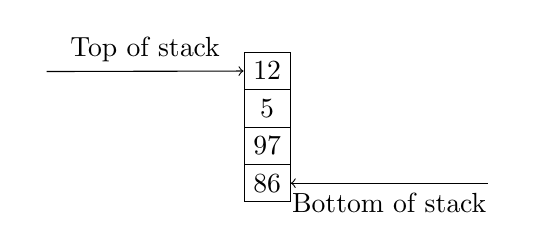
\begin{tikzpicture}[stack/.style={rectangle split, rectangle split parts=#1,draw, anchor=center}]
      \node (s4) [stack=4] {
      \nodepart{one}12
      \nodepart{two}5
      \nodepart{three}97
      \nodepart{four}86
      };
      \node (blank1) [above left=-0.375cm and 2.5cm of s4] {};
      \draw[->] (blank1) edge["Top of stack"] (s4.one west);
      \node (blank2) [right=2.5cm of s4.four east] {};
      \draw[->] (blank2) edge["Bottom of stack"] (s4.four east);
    \end{tikzpicture}
    \caption{Layout of a stack with four elements.}
    \label{fig:basicstack}
  \end{figure}


  \section{Adding an Item to a Stack}
  To add an item to a stack, the value is \emph{pushed} onto the top of the stack, making the value's position on the stack the new top.
  Figure~\ref{fig:pushtostack} shows a value being pushed onto a stack.
  \begin{figure}[h]
    \centering
    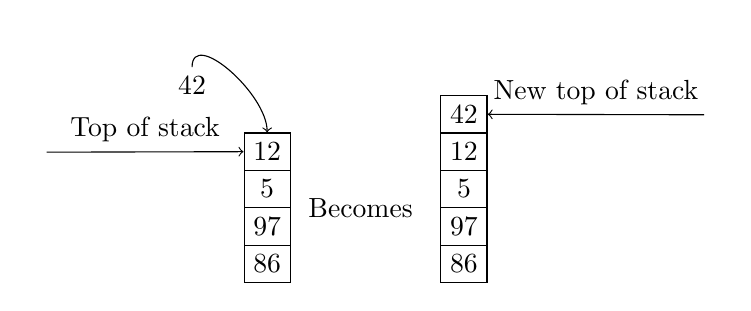
\begin{tikzpicture}[stack/.style={rectangle split, rectangle split parts=#1,draw}]
      \node (s4) [stack=4] {
      \nodepart{one}12
      \nodepart{two}5
      \nodepart{three}97
      \nodepart{four}86
      };
      \node (becomes) [right=0.1cm of s4] {Becomes};
      \node (blank1) [above left=-0.375cm and 2.5cm of s4] {};
      \draw[->] (blank1) edge["Top of stack"] (s4.one west);
      \node (item) [above left=.5cm of s4] {42};
      \draw[->] (item) to[out=90, in=90] (s4);
      \node[right=2.5cm of s4.south, anchor=south] (s5) [stack=5] {
      \nodepart[]{one}42
      \nodepart{two}12
      \nodepart{three}5
      \nodepart{four}97
      \nodepart{five}86
      };
      \node (blank2) [above right=-0.375cm and 2.75cm of s5] {};
      \draw[auto=right,->] (blank2) edge["New top of stack"] (s5.one east);
    \end{tikzpicture}
    \caption{Pushing the value~42 onto a stack.}
    \label{fig:pushtostack}
  \end{figure}

  \section{Removing an Item from a Stack}
  To remove an item from a stack, the item is \emph{popped} from the stack. If there is an item "under" the removed item, that item becomes the new top of the stack.
  Figure~\ref{fig:popfromstack} shows a value being popped off of a stack.
  \begin{figure}[h]
    \centering
    \begin{tikzpicture}[stack/.style={rectangle split, rectangle split parts=#1,draw}]
      \node (s5) [stack=5] {
      \nodepart[]{one}42
      \nodepart{two}12
      \nodepart{three}5
      \nodepart{four}97
      \nodepart{five}86
      };
      \node (becomes) [right=0.1cm of s4] {Becomes};
      \node (blank1) [above left=-0.375cm and 2.5cm of s5] {};
      \draw[->] (blank1) edge["Top of stack"] (s5.one west);
      \node (item) [above right=.5cm of s5] {42};
      \draw[->] (s5) to[out=90, in=90] (item);
      \node[right=2.5cm of s5.south, anchor=south] (s4) [stack=4] {
      \nodepart{one}12
      \nodepart{two}5
      \nodepart{three}97
      \nodepart{four}86
      };
      \node (blank2) [above right=-0.375cm and 2.75cm of s4] {};
      \draw[auto=right,->] (blank2) edge["New top of stack"] (s4.one east);
    \end{tikzpicture}
    \caption{Popping the top value off a stack.}
    \label{fig:popfromstack}
  \end{figure}
  Some stack implementations return the popped value, while others simply remove the topmost item and provide a separate operation to access the current top of the stack.

  \section{Additional Stack Operations.}
  In general, \emph{push} and \emph{pop} are the only two operations that are required of a stack data structure.

  As mentioned above, some implementations of a stack provide a \emph{peek}---or \emph{top}---operation to look at the current top of the stack. These implementations usually---but not always---simply remove the current top-most item when the pop operation is invoked.

  An implemtation might also provide a method to report the number of items currently on the stack, and possibly a method to determine whether the stack is empty.

  \section{Stack Usage}
  Use a stack when you need a last-in-first-out (LIFO) data structure.

  One example of using a stack is in validating the positions of brackets, braces, and parentheses in a string. For example the string
  \begin{verbatim}
    [bracket {brace (parentheses)}]\end{verbatim}
  is valid because each opening symbol has a matching closing symbol in the correct order. On the other hand,
  \begin{verbatim}
    [bracket {brace parentheses)}]\end{verbatim}
  is invalid because there is no opening parenthesis to match the closing symbol.

  We can write a small program that uses a stack to validate strings such as these. In \Cpp, such a program might look like this:
  \begin{lstc}[firstnumber=1]
#include <iostream>
#include <stack>  // The C++ library provides a stack type

// return true if the string is valid, false if it is not.
bool validate(const char *string)
{
  std::stack<char> stack;  // A stack of chars
  const char *p = string;

  while (*p)
  {
    // Each opening brace/bracket/parenthesis is stored in the stack
    if (*p == '[' || *p == '{' || *p == '(')
    {
      stack.push(*p);
    }
    else if (*p == ']' || *p == '}' || *p == ')')
    {
      if (stack.empty())
        return false;

      char  match = stack.top();

      if (match == '}' && *p != '{')
        return false;
      else if (match == ']' && *p != '[')
        return false;
      else if (match == ')' && *p != '(')
        return false;
      stack.pop();  // found a match, pop it off the stack.
    }
    ++p;
  }

  return stack.empty(); // There should be nothing left on the stack
}

int main()
{
  const char *strings[]
    {
      "{brace [bracket (paren)]}",
      "{brace [bracket paren)]}",
      "{brace [bracket (paren)]"
    };

  for (const char *s : strings)
  {
    std::cout << '"' << s << "\" ";
    if (validate(s))
      std::cout << "valid\n";
    else
      std::cout << "invalid\n";
  }

  return 0;
}\end{lstc}
  In this program we use the \textbf{stack} type provided by the \Cpp\ standard library with the \verb|#include <stack>| statement on line~2. Later we will implement our own stack type.

  The \verb|validate| function examines each character in the string passed to it. If the character is one of the opening bracket/brace/parenthesis characters, that character is pushed onto the stack (lines 13--16). Otherwise, if the character is one of the closing bracket/brace/parenthesis symbols (line~17), we first determine if the stack is empty. If it is empty, there are no opening symbols to compare against and the function returns \verb|false|.

  If there are still characters on the stack, we examine the character on the top of the stack. If the opening character on the stack does not match the coresponding closing character found in the string, the function returns \verb|false| (lines 22--29), otherwise it pops the matching character off the stack and examines the next character in the string.

  Once each character in the string has been checked, we once again look to see if the stack is empty, on line~35. If it is empty, we have matched all of the symbols in the string and we return \verb|true|. If the stack is not empty, there are still symbols on the stack that were not matched in the string, so we return \verb|false| to indicate that the string is not valid.

  Out test program's \verb|main| function simple loops over an array of strings, passing each to the \verb|validate| function and printing whether the string is valid or not. For the array of strings in \verb|main|, the output is
  \begin{verbatim}
    "{brace [bracket (paren)]}" valid
    "{brace [bracket paren)]}" invalid
    "{brace [bracket (paren)]" invalid
  \end{verbatim}

  \part{Implementation}\label{part:implementation}
  This part provides sample implementations of stacks, in both the C and \Cpp\ languages. The C program implements a bounded, fixed-size stack, using an array as the underlying data type, and is simple and straightforward, while the \Cpp\ implementation utilizes an Object Oriented Programming approach to create an unbounded stack utilizing a singly-linked list.
  \section{C Implementation}
  \label{sect:C_implementation}
  Here we present an implementation of a stack in the C language. This implementation uses simple integers for the type of data stored on the stack. The code can be easily modified to work with any data type.

  The implementation consists of two C source files, \verb|stack.h| and \verb|stack.c|. It begins in \verb|stack.h| with the definition of the structure and functions that provide the interface for our stack.
  \begin{lstc}[firstnumber=1]
typedef struct stack
{
  size_t  capacity; // max capacity of our fixed-size stack
  size_t  top;      // current position of the top of the stack
  int    *data;     // contents of the stack
} stack;

stack *stack_create(size_t capacity);
void stack_delete(stack *stack);
void stack_push(stack *stack, int value);
void stack_pop(stack *stack);
int stack_top(const stack *stack);
size_t stack_size(const stack *stack);
size_t stack_capacity(const stack *stack);
int stack_is_empty(const stack *stack);
int stack_is_full(const stack *stack);\end{lstc}
  The \verb|stack| structure contains information about our stack: in particular it stores the maximum capacity, the position of the top of the stack, and a pointer to the stack data. The \verb|stack_create| function will allocate memory and assign it to the \verb|data| pointer.

  The \verb|top| structure member is the index into the \verb|data| array of the current top of the stack. Since \verb|top| is an unsigned value, and zero is a valid array index, we will use zero in \verb|top| to indicate an empty stack, and a value one more than the current index for each stack position. This will be an internal detail and invisible to the user.

  This completes \verb|stack.h|. The function implementations are in \verb|stack.c|.

  The first thing to do is to \verb|#include| two standard C library header files. The file \verb|assert.h| defines the \verb|assert| macro which we will use for bounds checking. The file \verb|stdlib.h| file declares the \verb|malloc| and \verb|free| functions which we will use to allocate and free memory for our stack.

  Following the C library files, we \verb|#include| our \verb|stack.h| file that we looked at earlier.

  Next is the implementation code for the functions that operate on the stack, starting with \verb|stack_create|.
  \begin{lstc}[firstnumber=1]
stack *stack_create(size_t capacity)
{
  stack *new_stack = (stack *)malloc(sizeof(stack));
  if (new_stack == NULL)
    return NULL;

  new_stack->capacity = capacity;
  new_stack->top = (size_t)0;
  new_stack->data = (int *)malloc(capacity * sizeof(int));
  if (new_stack->data == NULL)
  {
    free(new_stack);
    return NULL;
  }

  return new_stack;
}\end{lstc}
  The \verb|capacity| parameter on line~1 specifies the maximum number of elements we can store in our stack. On line~3 we use the \verb|malloc| function to allocate memory for our stack structure. If the memory allocation fails, we return \verb|NULL| to indicate an error.

  Next, on line~7 we store the capacity in out \verb|stack| structure, then on line~8 we initialize the top-of-stack index to 0, indicating that the stack is empty.

  On line~9 we attempt to allocate memory for \verb|capacity| integers, and store the resultant pointer in the \verb|data| structure member. If the allocation fails, which we test for on line~10, then we make sure to free the memory we allocated to the structure (line~12) and again return \verb|NULL| to indicate an error in creating the stack. If our allocation succeeds, on line~16 we return a pointer to our stack.

  When we are done using our stack, we will want to free any memory allocated to it. The \verb|stack_delete| function on line~18 does this by first freeing the \verb|data| array, then freeing the memory for the stack structure itself.
  \begin{lstc}
void stack_delete(stack *stack)
{
  free(stack->data);
  free(stack);
}\end{lstc}

  The \verb|stack_push| function pushes a new value onto the stack
  \begin{lstc}
void stack_push(stack *stack, int value)
{
  assert(!stack_is_full(stack));

  stack->data[stack->top++] = value;
}\end{lstc}

  Line~25 assures the stack is not already at full capacity. In line~27 we store the pushed value at the current top of the stack and increment the \verb|top| index value. Note that \verb|top| is incremented \emph{after} the value is added to the array: this allows us to use a \verb|top| value of zero to indicate the stack is empty.

  The \verb|stack_pop| function removes the top-most item from the stack.
  \begin{lstc}
void stack_pop(stack *stack)
{
  assert(!stack_is_empty(stack));

  --stack->top;
}\end{lstc}
  Line~31 uses \verb|assert| to ensure the stack is not empty. Then line~33 simply decrements the top-of-stack index.

  Next, the \verb|stack_top| function returns the value at the top of the stack.
  \begin{lstc}
int stack_top(const stack *stack)
{
  assert(!stack_is_empty(stack));

  return stack->data[stack->top-1];
}\end{lstc}
  Again, \verb|assert| is used to ensure the stack is not empty. Line~39 returns the value at the top of the stack. Remember, the \verb|top| structure member always indexes the location one position beyond the top-most element of the array so we use \verb|top-1| to index the correct array element.

  The \verb|stack_size| function returns the number of items currently on the stack.
  \begin{lstc}
size_t stack_size(const stack *stack)
{
  return stack->top;
}\end{lstc}
  This function is very simple. It simply returns the \verb|top| member of the stack structure. Since \verb|top| always contains the array index one beyond the top-most item on the stack, it doubles as a counter.

  The \verb|stack_capacity| function is equally simple.
  \begin{lstc}
size_t stack_capacity(const stack *stack)
{
  return stack->capacity;
}\end{lstc}
  It returns the \verb|capacity| member of the stack structure. This is the same value passed as the stack capacity to the \verb|stack_create| function.

  Finally, we define the \verb|stack_is_empty| and \verb|stack_is_full| functions.
  \begin{lstc}
int stack_is_empty(const stack *stack)
{
  return stack->top == 0;
}
int stack_is_full(const stack *stack)
{
  return stack->top == stack->capacity;
}\end{lstc}
  We used these functions earlier. Line~51 in function \verb|stack_is_empty| returns a non-zero value if the \verb|top| structure member is equal to zero, indicating the stack is empty. Line~55 in the function \verb|stack_is_full| function returns a non-zero value if the \verb|top| structure member is equal to the stack capacity, indicating the stack is full.

  This completes the implementation of a fixed-size stack in C, produced in just~72 lines of code.

  \section{\texorpdfstring{\Cpp}{C++} Implementation}
  \label{sect:Cpp_implementation}
  This section presents an implementation of an unbounded stack in the \Cpp\ language. The implementation utilizes Object Oriented Programming principles, particularly encapsulation. Templates are also used so a stack can use any copyable data type.

  Note that this implementation in purely expositive. The \Cpp\ standard library provides an excellent stack implementation that is much more thoroughly optimized and tested, and should be preferred in production code.

  Unlike the C version, which employed two source files, a \verb|.h| header and a \verb|.c| source file, the \Cpp\ version will be implemented as header-only, using only a single \Cpp\ \verb|.h| header file.

  Like the C version, this implementation uses the \verb|assert| macro to handle errors. The definition of this macro is in the \verb|<cassert>| standard header file.
\begin{lstcpp}[firstnumber=1]
#include <cassert>\end{lstcpp}
  Next we begin the definition of the \verb|Stack| class. The entire implementation will be in this class.
\begin{lstcpp}
template <typename T>
class Stack
{\end{lstcpp}
  Class \verb|Stack| is a class template, so we will be able to use any copyable data type for the data stored in our stack.

  We will be implementing this stack using a singly-linked list as the underlying data type. A linked list is essentially a sequence of nodes, connected by pointers. For more information about linked lists, see this article: \url{https://github.com/jeffbi/data-structures/blob/master/LinkedList/doc/linkedlist.pdf}

  We first define our linked list node type:
\begin{lstcpp}
private:
  struct node
  {
    explicit node(const T& value)
      : _data{value},
        _next{nullptr}
    {}

    T     _data;
    node *_next;
  };\end{lstcpp}
  There are two data members of the \verb|node| structure: \verb|_data|, defined on line~13, is the actual data stored on the stack; \verb|_next|, defined on line~14, is a pointer to the next node in the linked list. The \verb|node| constructor, defined on lines~8--11, initializes the node with a data value and sets the \verb|_next| pointer to \verb|nullptr|.

  The \verb|Stack| has two data members:
  \begin{lstcpp}
  size_t  _size;
  node   *_head;\end{lstcpp}
  The \verb|_size| member stores the number of items currently on the stack, while the \verb|_head| member is a pointer to a \verb|node| and is the head node of our linked list. If the \verb|_head| pointer is the \verb|nullptr|, then the stack is empty. Otherwise this pointer points to the head of the linked list, which is also the top element of the stack.

  We now begin the public interface of the \verb|Stack| class. First, we provide a default constructor that initializes an empty stack, setting the \verb|_size| member to zero and the \verb|_head| member to \verb|nullptr|:
  \begin{lstcpp}
  Stack()
   : _size{0},
     _head{nullptr}
  {
  }\end{lstcpp}

  The destructor is the most complicated function in the \verb|Stack| class. It iterates over the linked list, head to tail (top of stack to bottom), and frees the memory allocated to each node:
  \begin{lstcpp}
  ~Stack()
  {
    while (_head)
    {
      node *new_head = _head->_next;
      delete _head;
      _head = new_head;
    }
  }\end{lstcpp}
  On line~25, so long as the \verb|_head| data member is not the \verb|nullptr|, the destructor stores a temporary copy of the \verb|_head|'s \verb|_next| pointer (line~27), deletes the memory allocated to the \verb|_head| linked list node (line~28) then re-assigns the \verb|_head| node to the copy of the previous \verb|_head|'s \verb|_next| pointer. This frees all the memory allocated to storing the stack data.

  The \verb|push| member function is how we get a new item onto the top of the stack.
  \begin{lstcpp}
  void push(const T &value)
  {
    node *new_head = new node(value);

    new_head->_next = _head;
    _head = new_head;

    ++_size;
  }\end{lstcpp}
  The \verb|value| parameter is the item we want to add to the top of the stack. On line~34 we create a new node with \verb|value|. Line~36 inserts the newly-created node as the new head of the list by setting the new head's \verb|_next| pointer to point to the current head (which will be the \verb|nullptr| if the stack is currently empty). Line~37 re-assigns the current \verb|_head| pointer to the new head. Finally, on line~39 we simply add one to the \verb|_size| data member. Note that we did not check to see if the stack is full. This stack implementation is unbounded so we can push as many item as we can create nodes for.

  The \verb|pop| member function removes the top-most item from the stack.
  \begin{lstcpp}
  void pop()
  {
    assert(!is_empty());
    node *old_head = _head;

    _head = old_head->_next;
    delete old_head;

    --_size;
  }\end{lstcpp}
  Here, we do care if the stack is empty. We cannot pop a value if there are no values on the stack, so the first thing we do is use \verb|assert| on line~43 to ensure that the stack is not empty. We then store a temporary copy of the stack's \verb|_head| pointer on line~44, reset the head to the old \verb|_head|'s \verb|_next| pointer on line~46, then delete the old head node (line~47). Finally we decrement the \verb|_size| data member to indicate that there is one less item on the stack.

  The \verb|top| function is used to see the value currently on the top of the stack.
  \begin{lstcpp}
  const T &top() const
  {
    assert(!is_empty());
    return _head->_data;
  }\end{lstcpp}
  Like the \verb|pop| function, we need to check if the stack is empty---we cannot look at a value that does not exist---so we again use \verb|assert| to ensure that the stack is not empty. We then, on line~54 simply return the value in the \verb|_data| member of the \verb|_head| node.

  There are actually two versions of the \verb|top| function. The one we saw above returns a |verb|const| reference, which cannot be modified. We also have a version that returns a non-\verb|const| reference, one that can be modified. Except for the function signatures, the two work exactly alike:
  \begin{lstcpp}
  T &top()
  {
    assert(!is_empty());
    return _head->_data;
  }\end{lstcpp}

  Next is the \verb|is_empty| function which simply determines if the stack is empty.
  \begin{lstcpp}
  bool is_empty() const noexcept
  {
    return _head == nullptr;
  }\end{lstcpp}
  For our purposes, the stack is empty if the \verb|_head| data member is equal to the \verb|nullptr|. Line~63 returns \verb|true| is that is the case, and \verb|false| otherwise.

  The final function in our stack implementation, \verb|size()|, returns the number of items on the stack, by returning the currently value of the \verb|_size| data member.
  \begin{lstcpp}
  size_t size() const noexcept
  {
    return _size;
  }\end{lstcpp}

  This completes the implementation of an unbounded stack in \Cpp, in under~70 lines of code.
\end{document}
